\documentclass[12pt,titlepage]{article}
\usepackage[margin=1.25in]{geometry}
\usepackage{graphicx,amsmath,enumitem,minted}

%% Variables definition
\newcommand{\vSubject}{Database}
\newcommand{\vSubtitle}{Midterm Exam}
\newcommand{\vName}{Dicha Zelianivan Arkana}
\newcommand{\vNIM}{2241720002}
\newcommand{\vClass}{1i}
\newcommand{\vDepartment}{Information Technology}
\newcommand{\vStudyProgram}{D4 Informatics Engineering}

%% [START] Tikz related stuff
\usepackage{tikz}
\usetikzlibrary{svg.path,calc,shapes.geometric,shapes.misc}
\tikzstyle{terminator} = [rectangle, draw, text centered, rounded corners = 1em, minimum height=2em]
\tikzstyle{preparation} = [chamfered rectangle, chamfered rectangle sep=0.75em, draw, text centered, minimum height = 2em]
\tikzstyle{process} = [rectangle, draw, text centered, minimum height=2em]
\tikzstyle{decision} = [diamond, aspect=2, draw, text centered, minimum height=2em]
\tikzstyle{data}=[trapezium, draw, text centered, trapezium left angle=60, trapezium right angle=120, minimum height=2em]
\tikzstyle{connector} = [line width=0.25mm,->]
%% [END] Tikz related stuff

%% [START] Fancy header related stuff
\usepackage{fancyhdr}
\pagestyle{fancy}
\setlength{\headheight}{15pt} % compensate fancyhdr style
\fancyhead{}
\fancyfoot{}
\fancyfoot[L]{\thepage}
\fancyfoot[R]{\textit{\vSubject - \vSubtitle}}
\renewcommand{\footrulewidth}{0.4pt}% default is 0pt, overline for footer
%% [END] Fancy header related stuff

%% [START] Custom tabular command related stuff
\usepackage{tabularx}
\newcommand{\details}[2]{
    #1 & #2  \\
}
%% [END] Custom tabular command related stuff

%% [START] Figure related stuff
\newcommand{\image}[3][1]{
    \begin{figure}[h]
        \centering
        \includegraphics[#1]{#2}
        \caption{#3}
        \label{#3}
    \end{figure}
}
%% [END] Figure related stuff

\begin{document}
\begin{titlepage}
    \centering
    \vfill
    {\bfseries\LARGE
        \vSubject\\
        \vskip0.25cm
        \vSubtitle
    }
    \vfill
    
\includegraphics[width=6cm]{images/polinema-logo.png}
    \vfill
    {
        \textbf{Name}\\
        \vName\\
        \vskip0.5cm
        \textbf{NIM}\\
        \vNIM\\
        \vskip0.5cm
        \textbf{Class}\\
        \vClass\\
        \vskip0.5cm
        \textbf{Department}\\
        \vDepartment\\
        \vskip0.5cm
        \textbf{Study Program}\\
        \vStudyProgram
    }
\end{titlepage}

\section{Analysis}
\begin{enumerate}[label=\alph*.)]
    \item {
        Create the Entity-Relationship Diagram for the following business rule, assume relevant attributes

        \begin{figure}[h]
            \centering
            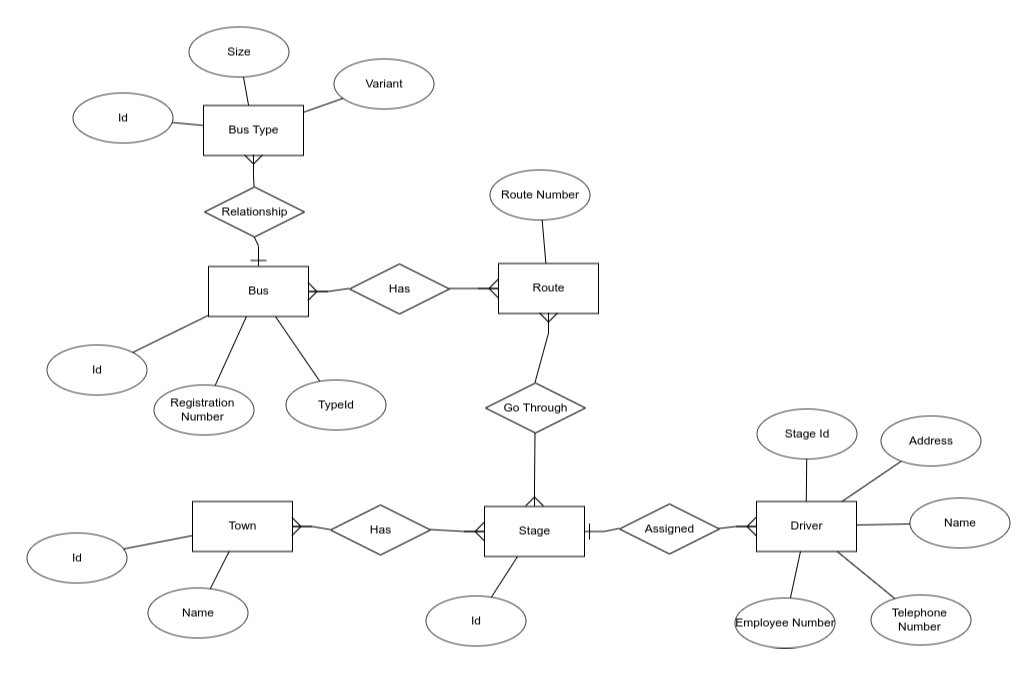
\includegraphics[width=.65\textwidth]{./images/erdplus.png}
            \caption{The Entity Relationship Diagram for the problem}
        \end{figure}
    }
    \item {
        Transform the ERD into Relational Schema

        \begin{figure}[h]
            \centering
            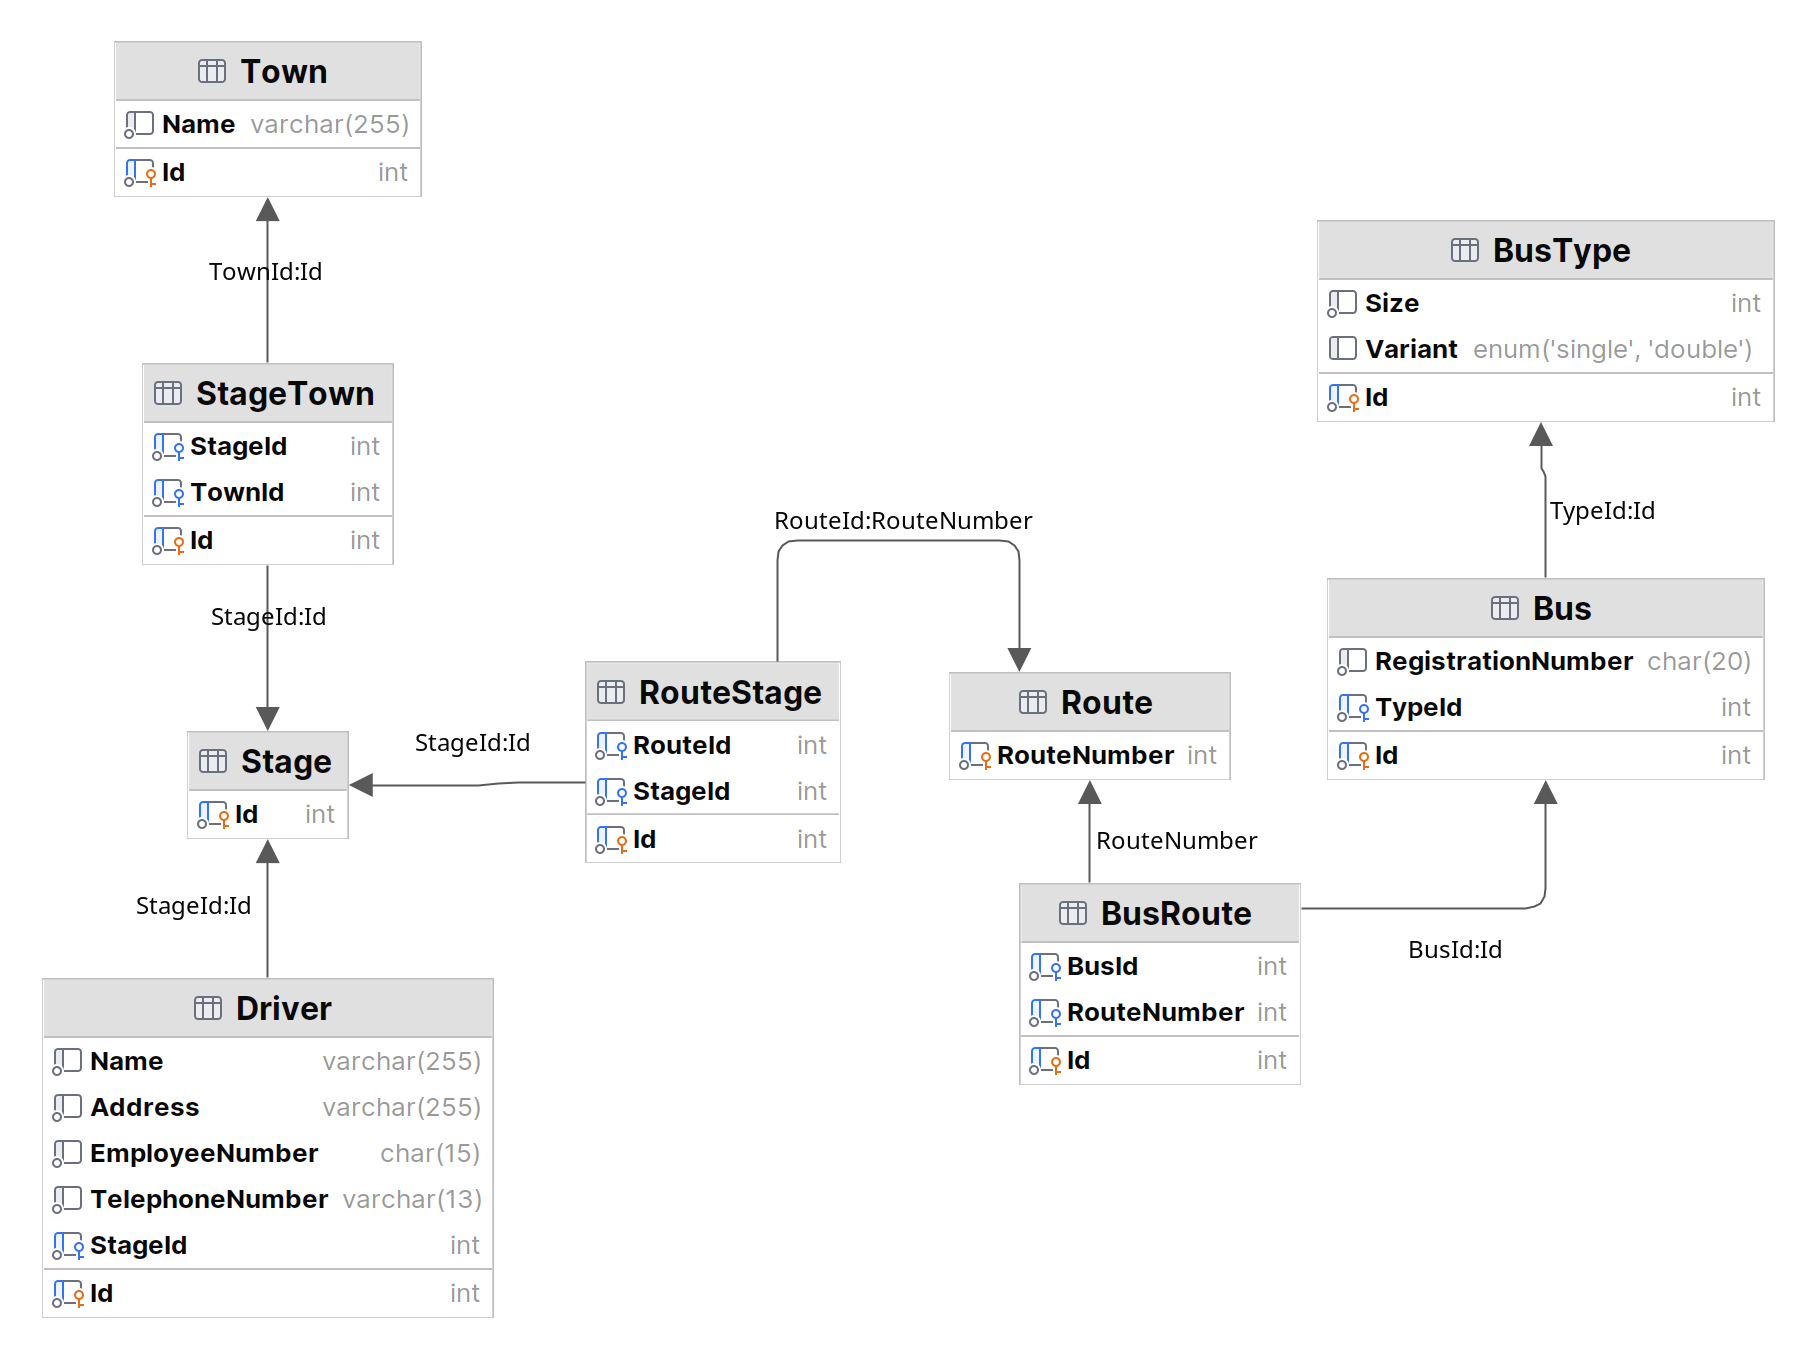
\includegraphics[width=.65\textwidth]{./images/erd.png}
            \caption{The relational version of the diagram}
        \end{figure}

        \pagebreak

        \large{\textbf{Query Steps}}
        \begin{itemize}
            \item {
                Create the database and use it as the default schema.

                \begin{minted}[autogobble,fontsize=\small]{sql}
                    CREATE DATABASE bus_system;
                    USE bus_system;
                \end{minted}
            }
            \item {
                Create the tables

                \begin{minted}[autogobble,fontsize=\small]{sql}
                    CREATE TABLE Bus
                    (
                        Id                 INT      NOT NULL PRIMARY KEY AUTO_INCREMENT,
                        RegistrationNumber CHAR(20) NOT NULL,
                        TypeId             INT      NOT NULL
                    );

                    CREATE TABLE BusType
                    (
                        Id      INT NOT NULL PRIMARY KEY AUTO_INCREMENT,
                        Size    INT NOT NULL,
                        Variant ENUM ('single', 'double') DEFAULT ('single')
                    );

                    CREATE TABLE BusRoute
                    (
                        Id          INT NOT NULL PRIMARY KEY AUTO_INCREMENT,
                        BusId       INT NOT NULL,
                        RouteNumber INT NOT NULL
                    );

                    CREATE TABLE Route
                    (
                        RouteNumber INT NOT NULL PRIMARY KEY AUTO_INCREMENT
                    );

                    CREATE TABLE RouteStage
                    (
                        Id      INT NOT NULL PRIMARY KEY AUTO_INCREMENT,
                        RouteId INT NOT NULL,
                        StageId INT NOT NULL
                    );

                    CREATE TABLE Stage
                    (
                        Id INT NOT NULL PRIMARY KEY AUTO_INCREMENT
                    );

                    CREATE TABLE StageTown
                    (
                        Id      INT NOT NULL PRIMARY KEY AUTO_INCREMENT,
                        StageId INT NOT NULL,
                        TownId  INT NOT NULL
                    );

                    CREATE TABLE Town
                    (
                        Id   INT          NOT NULL PRIMARY KEY AUTO_INCREMENT,
                        Name VARCHAR(255) NOT NULL
                    );

                    CREATE TABLE Driver
                    (
                        Id              INT          NOT NULL PRIMARY KEY AUTO_INCREMENT,
                        Name            VARCHAR(255) NOT NULL,
                        Address         VARCHAR(255) NOT NULL,
                        EmployeeNumber  CHAR(15)     NOT NULL,
                        TelephoneNumber VARCHAR(13)  NOT NULL,
                        StageId         INT          NOT NULL
                    );
                \end{minted}
            }
            \item {
                Create relationships

                \begin{minted}[autogobble,fontsize=\small]{sql}
                    ALTER TABLE Bus
                        ADD FOREIGN KEY (TypeId) REFERENCES BusType (Id);
                    ALTER TABLE BusRoute
                        ADD FOREIGN KEY (BusId) REFERENCES Bus(Id);
                    ALTER TABLE BusRoute
                        ADD FOREIGN KEY (RouteNumber) REFERENCES Route(RouteNumber);
                    ALTER TABLE StageTown
                        ADD FOREIGN KEY (StageId) REFERENCES Stage (Id);
                    ALTER TABLE StageTown
                        ADD FOREIGN KEY (TownId) REFERENCES Town (Id);
                    ALTER TABLE RouteStage
                        ADD FOREIGN KEY (RouteId) REFERENCES Route (RouteNumber);
                    ALTER TABLE RouteStage
                        ADD FOREIGN KEY (StageId) REFERENCES Stage (Id);
                    ALTER TABLE Driver
                        ADD FOREIGN KEY (StageId) REFERENCES Stage (Id);
                \end{minted}
            }
        \end{itemize}
    }
\end{enumerate}

\pagebreak

\section{Application}
\begin{enumerate}[label=\Alph*.]
    \item {
        \large{\textbf{DDL Query}}

        \begin{minted}[autogobble,fontsize=\small]{sql}
            CREATE TABLE EMPLOYEE
            (
                Id      INT          NOT NULL PRIMARY KEY AUTO_INCREMENT,
                Fname   VARCHAR(255) NOT NULL,
                Lname   VARCHAR(255) NOT NULL,
                Ssn     CHAR(9)      NOT NULL,
                BDate   DATETIME     NOT NULL,
                Address VARCHAR(255) NOT NULL,
                Salary  INT          NOT NULL,
                Dno     INT          NOT NULL
            );

            CREATE TABLE PROJECT
            (
                Id        INT          NOT NULL PRIMARY KEY AUTO_INCREMENT,
                Pname     VARCHAR(255) NOT NULL,
                Plocation VARCHAR(255) NOT NULL,
                Pnumber   INT          NOT NULL,
                Dnum      INT          NOT NULL
            );

            CREATE TABLE DEPENDENT
            (
                Id             INT          NOT NULL PRIMARY KEY AUTO_INCREMENT,
                Essn           CHAR(9)      NOT NULL,
                Dependent_name VARCHAR(255) NOT NULL,
                Relationship   ENUM ('Daughter', 'Spouse', 'Son')
            );

            CREATE TABLE DEPARTMENT
            (
                Id             INT          NOT NULL PRIMARY KEY AUTO_INCREMENT,
                Dname          VARCHAR(255) NOT NULL,
                Dnumber        INT          NOT NULL,
                Mgr_ssn        CHAR(9)      NOT NULL,
                Mgr_start_date DATETIME     NOT NULL
            );
        \end{minted}
    }
    \pagebreak
    \item {
        \large{\textbf{Query Result}}
        
        \begin{figure}[h]
            \centering
            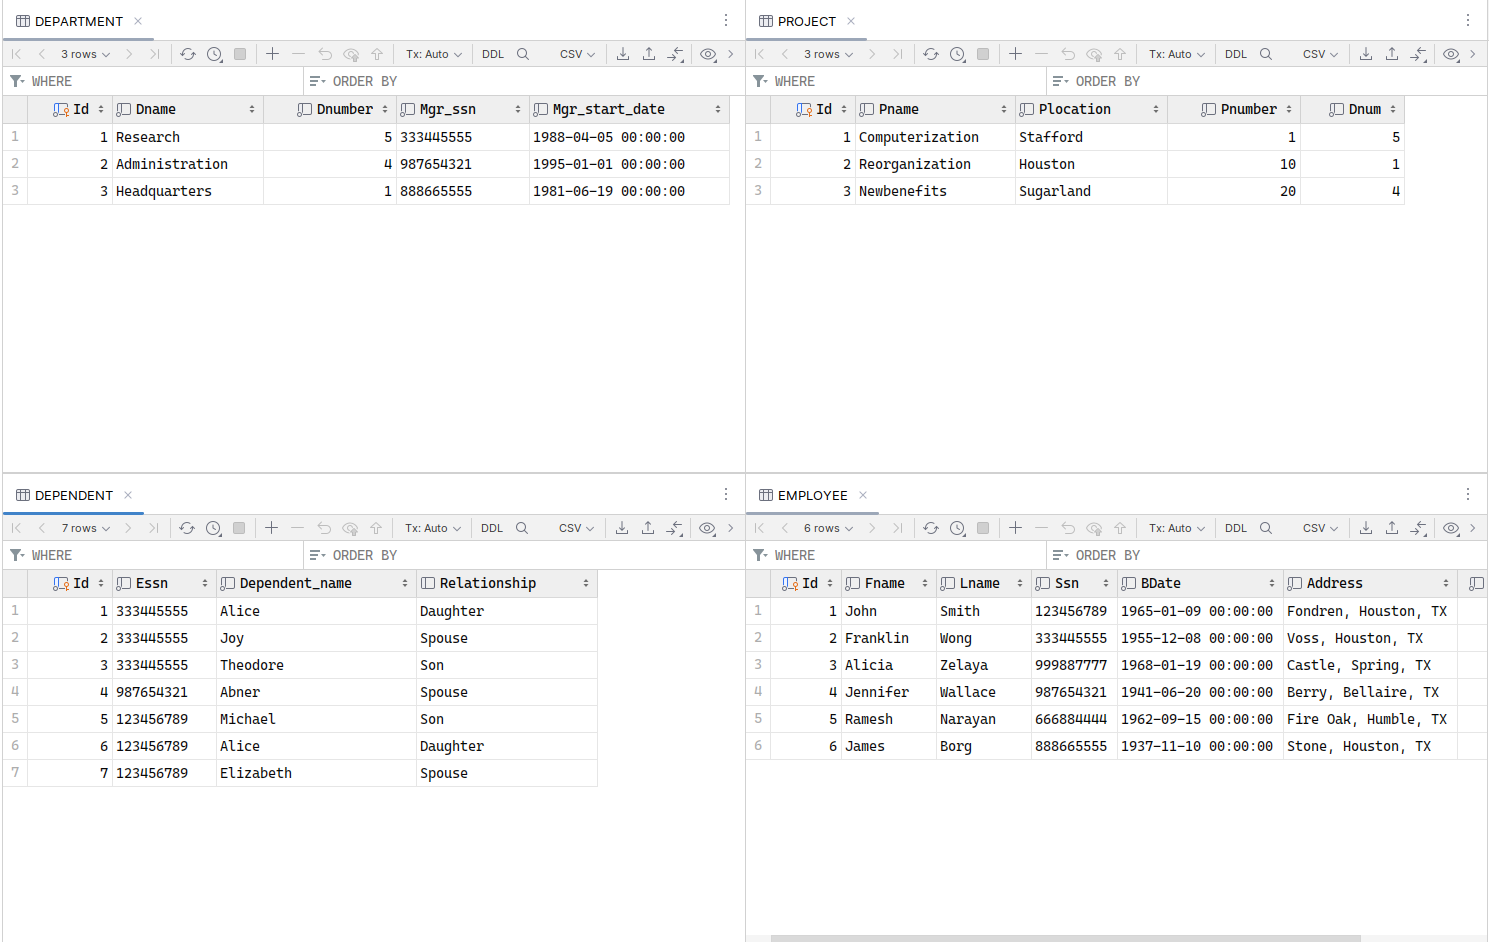
\includegraphics[width=\textwidth]{./images/db_tables.png}
            \caption{The result of the DDL queries above}
        \end{figure}
    }
\end{enumerate}

\subsection{Questions}

\begin{enumerate}[label=\Alph*.]
    \item {
        Create the SQL command to satisfy the following queries. Write at the space provided.

        \begin{enumerate}[label={\arabic*.}]
            \item {
                Find all information about John Smith

                \begin{minted}[autogobble,fontsize=\small]{sql}
                SELECT * FROM EMPLOYEE WHERE Fname='John' AND Lname='Smith';
                \end{minted}

                \begin{figure}[h]
                    \centering
                    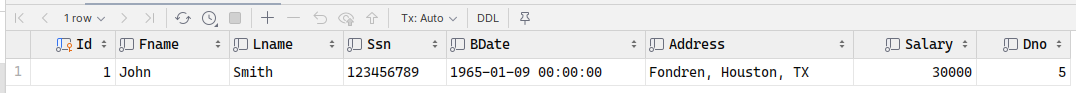
\includegraphics[width=.7\textwidth]{./images/output_1.png}
                \end{figure}
            }
            \pagebreak
            \item {
                What department started on 5 April, 1998?

                \begin{minted}[autogobble,fontsize=\small]{sql}
                SELECT Dname FROM DEPARTMENT WHERE Mgr_start_date='1988-04-05';
                \end{minted}

                \begin{figure}[h]
                    \centering
                    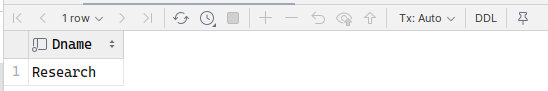
\includegraphics[width=.7\textwidth]{./images/output_2.png}
                \end{figure}
            }   
            \item {
                Where does James Borg lives?

                \begin{minted}[autogobble,fontsize=\small]{sql}
                SELECT Address FROM EMPLOYEE WHERE Fname='James' AND Lname='Borg';
                \end{minted}

                \begin{figure}[h]
                    \centering
                    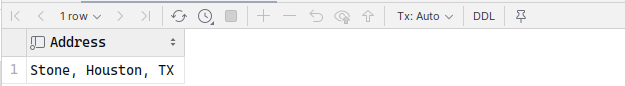
\includegraphics[width=.7\textwidth]{./images/output_3.png}
                \end{figure}
            }
            \item {
                Who are the spouses of the employees?

                \begin{minted}[autogobble,fontsize=\small]{sql}
                SELECT Dependent_name FROM DEPENDENT WHERE Relationship='Spouse';
                \end{minted}

                \begin{figure}[h]
                    \centering
                    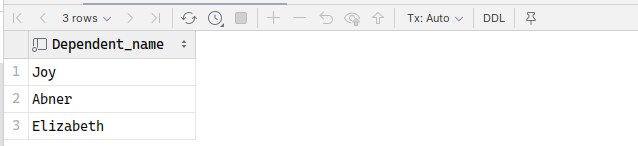
\includegraphics[width=.7\textwidth]{./images/output_4.png}
                \end{figure}
            }
            \item {
                What is the project located at Sugarland?

                \begin{minted}[autogobble,fontsize=\small]{sql}
                SELECT Pname FROM PROJECT WHERE Plocation='Sugarland';
                \end{minted}

                \begin{figure}[h]
                    \centering
                    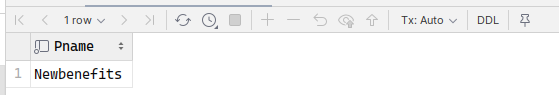
\includegraphics[width=.7\textwidth]{./images/output_5.png}
                \end{figure}
            }
        \end{enumerate}
    }
    \pagebreak
    \item {
        Create the SQL command to satisfy the following queries connecting different tables.
        \begin{enumerate}[label={\arabic*.}]
            \setcounter{enumii}{5}
            \item {
                Who is the manager of Research department?

                \begin{minted}[autogobble,fontsize=\small]{sql}
                SELECT
                    Fname, Lname
                FROM DEPARTMENT
                JOIN EMPLOYEE 
                ON DEPARTMENT.Mgr_ssn=EMPLOYEE.Ssn
                WHERE Dname='Research';
                \end{minted}

                \begin{figure}[h]
                    \centering
                    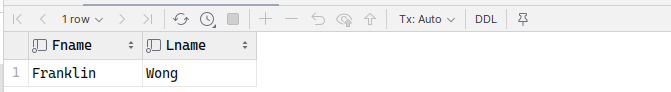
\includegraphics[width=.8\textwidth]{./images/output_6.png}
                \end{figure}
            }
            \item {
                Who are the employees that work on project newbenefits?

                \begin{minted}[autogobble,fontsize=\small]{sql}
                SELECT
                    Fname, Lname
                FROM PROJECT
                JOIN EMPLOYEE ON PROJECT.Dnum=EMPLOYEE.Dno
                WHERE Pname='Newbenefits';
                \end{minted}

                \begin{figure}[h]
                    \centering
                    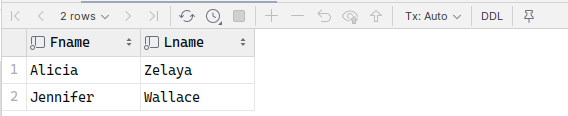
\includegraphics[width=.8\textwidth]{./images/output_7.png}
                \end{figure}
            }
            \pagebreak
            \item {
                Who are dependents of Franklin Wong?

                \begin{minted}[autogobble,fontsize=\small]{sql}
                SELECT
                    Dependent_name
                FROM DEPENDENT
                JOIN EMPLOYEE
                ON EMPLOYEE.Ssn=DEPENDENT.Essn
                WHERE Fname='Franklin' AND Lname='Wong';
                \end{minted}

                \begin{figure}[h]
                    \centering
                    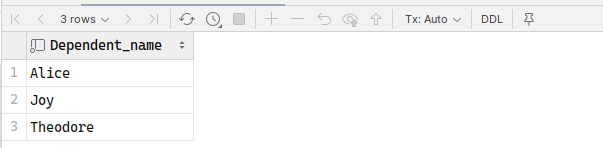
\includegraphics[width=.8\textwidth]{./images/output_8.png}
                \end{figure}
            }
            \item {
                Who are the dependents of employees who're assigned to project 'Computerization'?

                \begin{minted}[autogobble,fontsize=\small]{sql}
                SELECT
                    Dependent_name
                FROM DEPENDENT
                JOIN EMPLOYEE
                ON DEPENDENT.Essn=EMPLOYEE.Ssn
                JOIN PROJECT
                ON PROJECT.Dnum=EMPLOYEE.Dno
                WHERE Pname='Computerization';
                \end{minted}

                \begin{figure}[h]
                    \centering
                    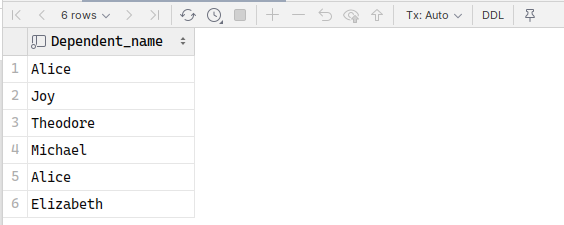
\includegraphics[width=.8\textwidth]{./images/output_9.png}
                \end{figure}
            }
            \pagebreak
            \item {
                In what department do employees belong, who's dependent are their sons?

                \begin{minted}[autogobble,fontsize=\small]{sql}
                SELECT
                    Dname
                FROM DEPARTMENT
                JOIN EMPLOYEE
                ON DEPARTMENT.Dnumber=EMPLOYEE.Dno
                JOIN DEPENDENT
                ON DEPENDENT.Essn=EMPLOYEE.Ssn
                WHERE Relationship='Son';
                \end{minted}

                \begin{figure}[h]
                    \centering
                    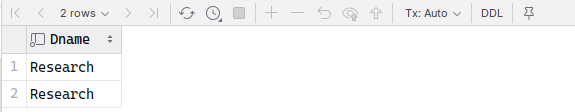
\includegraphics[width=.8\textwidth]{./images/output_10.png}
                \end{figure}
            }
        \end{enumerate}
    }
\end{enumerate}


\end{document}

